\documentclass{article}
\usepackage{graphicx}
\usepackage{amssymb}
\begin{document}

\title{Reactor Simulator: Transport Theory}

\author{Nicholas F. Herring\\
North Carolina State University}

\date{August 2017}

\maketitle

\section{Ray Tracing Theory}
\subsection{Cell Numbering Method}

The method of cell numbering in the program is based off of four different parameters

\begin{enumerate}
\item Radial section number $l=1, 2, 3, \dots, L$
\item Octant number $i=1, 2, 3, \dots, 8$
\item Pincell ``column" number $n=1, 2, 3, \dots, N$
\item Pincell ``row" number $m=1, 2, 3, \dots, M$
\end{enumerate}

The total cell number is determined by the following equation:
\begin{equation}
 c=i+8(l-1)+8 L(n-1)+8 LN(m-1)
 \label{eq:cellnumber}
\end{equation}

Figure \ref{fig:pincell} shows the numbering system of the first pincell in action. The cells are numbered from the bottom left outside of the pin cell, circling clockwise and going inward.

\begin{figure}[h]
\begin{center}
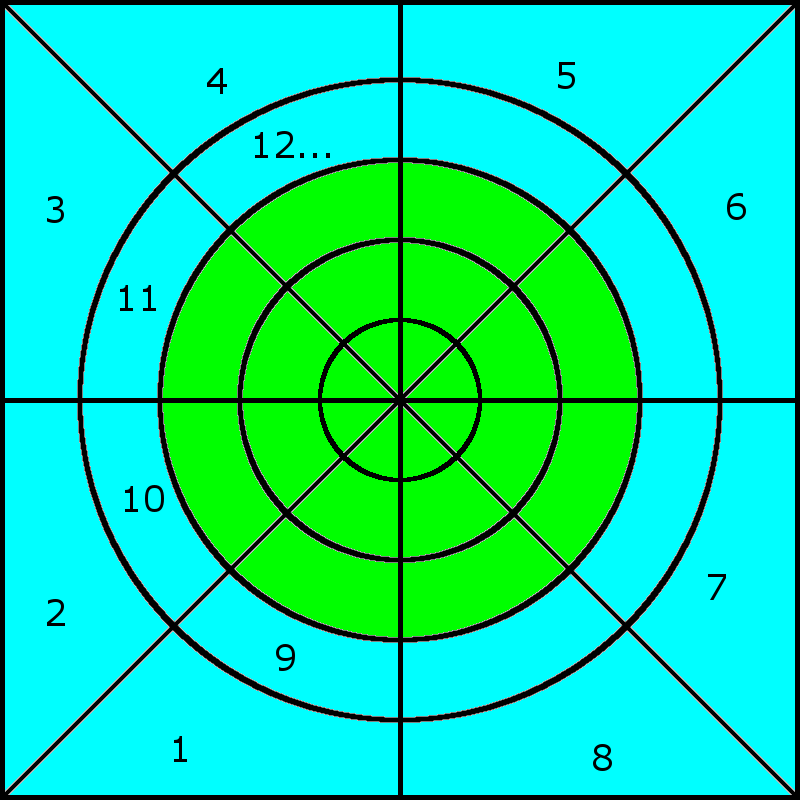
\includegraphics[width=40mm]{pincell.png}
\caption{Pincell numbering system}
\end{center}
\label{fig:pincell}
\end{figure}

Figure \ref{fig:pingrid} shows the numbering system for the assembly of pins. The value of the row number goes upwards from 1 at the bottom. The column number goes right from 1 at the far left.

\begin{figure}[h]
\begin{center}
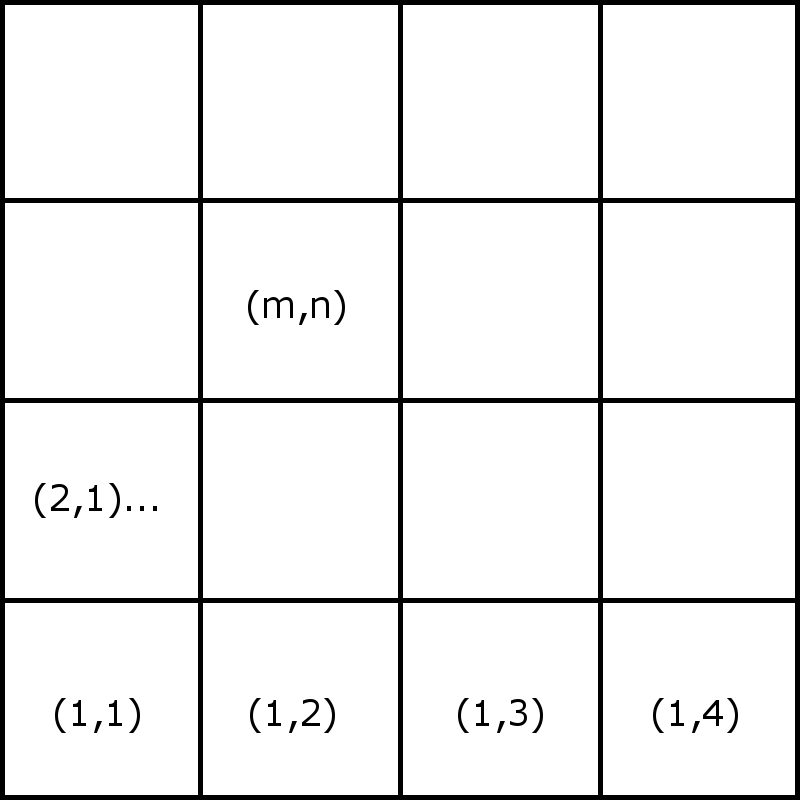
\includegraphics[width=40mm]{pingrid.png}
\caption{Assembly Numbering System}
\end{center}
\label{fig:pingrid}
\end{figure}

Pins are assumed to all be square with a user defined width of $\Delta$. Each pin is divided into $L$ radial sections, which means it has $L-1$ dividing circles of radius $r_l$ for $l=1,2,\dots,L-1$ where $r_L=0$ and $r_0=\infty$ by definition.

\subsection{Determining the Cell Number Containing a Point}

For a point $(x,y)$ in the domain of the problem, the cell that $(x,y)$ belongs to can be determined as follows.

To determine the grid ``column'' the following equation is solved for the integer $n$:
\begin{equation}
\Delta (n-1)<x<\Delta n
\label{eq:nsolution}
\end{equation}

To determine the grid ``row'' the following equation is solved for the integer $m$:
\begin{equation}
\Delta (m-1)<y<\Delta m
\label{eq:msolution}
\end{equation}

To simplify when determining the radial number $l$ and the octant number $i$, the location variables $(x,y)$ are transformed to $(\tilde{x},\tilde{y})$ by a cordinate transform to make the pincell $(m,n)$, that point $(x,y)$ belongs to, centered about the transformed cordinate system's origin, $(0,0)$. This is done by the following equations:
\begin{equation}
\tilde{x}=x-\Delta (n-1/2)
\label{eq:xtransform}
\end{equation}
\begin{equation}
\tilde{y}=y-\Delta (m-1/2)
\label{eq:ytransform}
\end{equation}

After this transform has been applied, the radial cell $l$ can be determined by solving the following equation for the integer $l$:
\begin{equation}
r_l<\sqrt{\tilde{x}^2+\tilde{y}^2}<r_{l-1}
\label{eq:lsolution}
\end{equation}

The determination of the octant number is slightly more complicated, and is solved by the following elimination logic:

\vspace{5mm}
\texttt{If} $\frac{|\tilde{x}|}{|\tilde{y}|} > 1$ \texttt{then}

\qquad $i\ne 2, 3, 6, 7$

\texttt{else}

\qquad $i\ne 1, 4, 5, 8$

\texttt{If} $\tilde{x} > 0$ \texttt{then}

\qquad $i\ne 1, 2, 3, 4$

\texttt{else}

\qquad $i\ne 5, 6, 7, 8$

\texttt{If} $\tilde{y} > 0$ \texttt{then}

\qquad $i\ne 1, 2, 7, 8$

\texttt{else}

\qquad $i\ne 3, 4, 5, 6$
\begin{equation}
\label{eq:isolution}
\end{equation}

With equations \ref{eq:nsolution}--\ref{eq:isolution}, the proper value of the actual cell number $c$ can be determined by equation \ref{eq:cellnumber}.

\subsection{Step Convergent Ray Tracing}

With the ability to determine which cell a point $(x,y)$ is in, the ray can now be traced by stepping along the characteristic curves. These curves are started from the edges of the domain with discrete angles determined by the chosen quadrature set of form $(\gamma_k,\theta_k,\omega_k)$ for $k=1,2,\dots,K$. Where $0<\gamma_k<180$, $0<\theta_k<90$, and $\sum_{k=1}^K\omega_k=2\pi$. The coordinate system associated with these angles is shown in Figure \ref{fig:anglecords}:

\begin{figure}[h]
\begin{center}
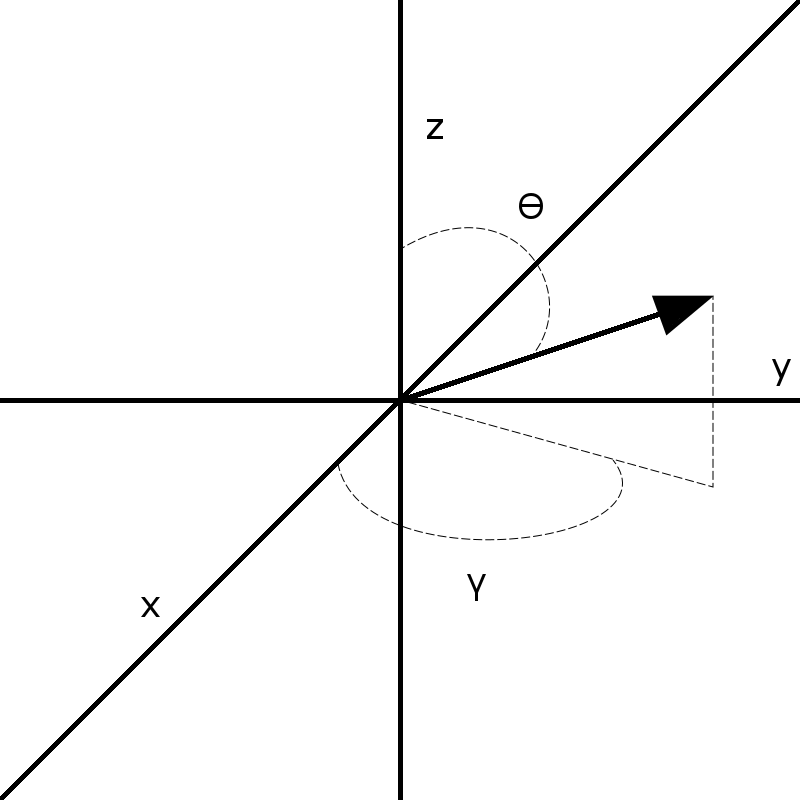
\includegraphics[width=40mm]{coordinates.png}
\caption{Angle Cordinates System}
\end{center}
\label{fig:anglecords}
\end{figure}

The rays are begun at points separated by the ray width $h$ along a line orthogonal to the characteristic curves (note that it is required here that $\Delta~ /h \in~ \mathbb{Z}$). The rays are started from the left, right, and bottom sides of the domain. Left and bottom for $\gamma>90$, and right and bottom for $\gamma<90$. A trivial proof, not to be repeated here, shows the spacing along the side can be calculated geometrically, for the curves starting on the left side, the spacing $s$ is given by:
\begin{equation}
s=\frac{h}{\cos({\gamma})}
\label{eq:leftpsacing}
\end{equation}

For curves starting from the right side, the spacing $s$ is given by:
\begin{equation}
s=\frac{h}{-\cos({\gamma})}
\label{eq:rightspacing}
\end{equation}

For curves starting from the bottom side, the spacing $s$ is given by:
\begin{equation}
s=\frac{h}{\sin({\gamma})}
\label{eq:botspacing}
\end{equation}

Once the rays are started, they are stepped through by the default step size $\xi=\frac{\Delta}{2}-2\epsilon \Delta$. 

\end{document}













